\documentclass[xcolor=dvipsnames]{beamer}

%%%%%%%%%%%%%%%%%%%%%%%%%%%%%%%
% PACKAGES
%%%%%%%%%%%%%%%%%%%%%%%%%%%%%%%

\usepackage{ucs}
\usepackage[utf8x]{inputenc}
\usepackage[english,russian]{babel}

\usepackage{eulervm} % use Euler VM font for math

\usepackage{ifdraft}

\usepackage{xspace}

\usepackage{algpseudocode}
\newcommand{\algorithmictitle}[1]{\hspace{8mm}\textbf{#1}}
\algrenewcommand{\algorithmiccomment}[1]{\hfill #1}

\usepackage{ulem}
\let\oldsout\sout
\renewcommand{\sout}[1]{\text{\oldsout{\ensuremath{#1}}}}
\renewcommand<>{\sout}[1]{\alt#2{\beameroriginal{\sout}{#1}}{#1}}

\usepackage{../../common/cypokcommon}

%%%%%%%%%%%%%%%%%%%%%%%%%%%%%%%
% DOCUMENT-SPECIFIC COMMANDS
%%%%%%%%%%%%%%%%%%%%%%%%%%%%%%%

% Provide some basic information about current Git revision.
%
% TODO: merge with gitinfo package?
% http://www.ctan.org/tex-archive/macros/latex/contrib/gitinfo

\InputIfFileExists{../../common/gitinfo-data}{}{
  % defaults
  \newcommand{\GitMissing}{(no Git info)}
  \newcommand{\GitAbbrHash}{\GitMissing}
  \newcommand{\GitDate}{\GitMissing}
  \newcommand{\GitSubject}{\GitMissing}
}



% add frame number to footline
\newcommand*\oldinsertshorttitle{}
\let\oldinsertshorttitle\insertshorttitle
\renewcommand*\insertshorttitle{
  \oldinsertshorttitle \hfill
  \insertframenumber\,/\,\inserttotalframenumber
}

\newenvironment{backup}
  {
    \appendix
    \newcounter{framenumberappendix}
    \setcounter{framenumberappendix}{\value{framenumber}}
  }
  {
    \addtocounter{framenumberappendix}{-\value{framenumber}}
    \addtocounter{framenumber}{\value{framenumberappendix}}
  }

% hide navigation symbols
\beamertemplatenavigationsymbolsempty

\newcommand{\java}{\eng{Java}\xspace}

\newcommand{\M}{\ensuremath{\mathbf{M}}}
\newcommand{\Mfield}[1]{\ensuremath{\mathbf{#1}}}

\newcommand{\type}[1]{\mathsf{#1}}
\newcommand{\field}[1]{\mathsf{#1}}
\newcommand{\sfield}[2]{\type{#1}.\field{#2}}
\newcommand{\method}[1]{\mathsf{#1}}

\newcommand{\op}[1]{\mathbf{#1}}
\newcommand{\pts}[1]{\widebar{#1}}

%%%%%%%%%%%%%%%%%%%%%%%%%%%%%%%
% SLIDES FORMAT
%%%%%%%%%%%%%%%%%%%%%%%%%%%%%%%

\usetheme{Warsaw}
\usecolortheme{seahorse}

\setbeamercovered{transparent}

%%%%%%%%%%%%%%%%%%%%%%%%%%%%%%%
% BODY
%%%%%%%%%%%%%%%%%%%%%%%%%%%%%%%

\title[Анализ указателей и синонимов]{
  Применение анализа указателей и синонимов
  для оптимизации многопоточных программ
}
\author[Парфиненко Владимир Владимирович]{
  Парфиненко Владимир Владимирович
  \texorpdfstring{%
    \\
    \vspace{0.5cm}
    \small
      Научные руководители:\\
      м.\,н.\,с.~ИСИ~СО~РАН, Павлов~Павел~Евгеньевич \\
      зав.\,лаб.~ИСИ~СО~РАН, к.\,т.\,н.~Шелехов~Владимир~Иванович
  }{}% short title in pdf
}
\institute{
  Новосибирский Государственный Университет
}
\date{
  Новосибирск, 2013\ifdraft{ \\\medskip \footnotesize Git date: \GitDate.}{}
}

\begin{document}

\begin{frame}
  \titlepage
\end{frame}

\begin{frame}{Анализ синонимов и указателей}

  \begin{block}{Анализ синонимов \engdef{Alias Analysis}}
    Могут ли два разных выражения ссылочного типа указывать на одно и то же
    место в памяти?
  \end{block}

  \begin{block}{Анализ указателей \engdef{Points-To Analysis}}
    На какие объекты в памяти могут указывать выражения ссылочного типа?
  \end{block}

\end{frame}

\begin{frame}{Цель и задачи}

  \begin{itemize}
    \item \textbf{Цель:}
          разработка алгоритма анализа указателей для языка \java
    \medskip
    \item \textbf{Основные задачи:}
      \begin{itemize}
        \item изучить существующие алгоритмы и разработать новый, выбрав
              подходящий за основу
        \item разработать схему выражения неявных зависимостей по памяти
      \end{itemize}
  \end{itemize}

\end{frame}

\begin{frame}{Недостатки предыдущей работы}

  \begin{center}
    \begin{minipage}[t]{0.60\textwidth}
      \begin{block}{Проблема с полями}
        \begin{algorithmic}[1]
          \State $x \gets \op{new}~\type{T}$
          \State $x.f \gets \op{new}~\type{Object}$
          \State $a \gets x.f$
          \State $x.f \gets \op{new}~\type{Object}$
          \State $b \gets x.f$
        \end{algorithmic}
      \end{block}
    \end{minipage}

    \medskip
    $a$ и $b$~--- могут ли быть синонимами?

    \visible<2->{Да.}
  \end{center}

\end{frame}

\begin{frame}{Суть нечувствительного к потоку управления анализа}

  \centerline{В\'{и}дение программы анализом, который к потоку управления \ldots}

  \begin{columns}[t]
    \begin{column}{0.5\textwidth}
      \begin{block}{\ldots чувствителен}
        \begin{algorithmic}[1]
          \State $x \gets \op{new}~\type{T}$
          \State $x.f \gets \op{new}~\type{Object}$
          \State $a \gets x.f$
          \State $x.f \gets \op{new}~\type{Object}$
          \State $b \gets x.f$
        \end{algorithmic}
      \end{block}
    \end{column}
    \begin{column}{0.5\textwidth}
      \begin{block}{\ldots нечувствителен}
        \begin{algorithmic}
          \State $x \gets \op{new}~\type{T}$
          \State $x.f \gets \op{new}~\type{Object}$
          \State $x.f \gets \op{new}~\type{Object}$
          \State $a \gets x.f$
          \State $b \gets x.f$
        \end{algorithmic}
      \end{block}
    \end{column}
  \end{columns}

\end{frame}

\begin{frame}{\M"=переменная}

  \begin{columns}[t]
    \begin{column}{0.4\textwidth}
      \begin{block}{Исходная программа}
        \begin{algorithmic}[1]
          \State $u \gets a.\field{f}$
          \If{(\ldots)}
            \State $a.\field{f} \gets x$
          \Else
            \State $a.\field{f} \gets y$
          \EndIf
          \State
          \State $v \gets a.\field{f}$
        \end{algorithmic}
      \end{block}
    \end{column}
    \begin{column}{0.6\textwidth}
      \begin{block}{Программа с \M"=переменной}
        \begin{algorithmic}
          \State $u \gets \op{getfield}(\M_0, a, \field{f})$
          \If{(\ldots)}
            \State $\M_1 \gets \op{putfield}(\M_0, a, \field{f}, x)$
          \Else
            \State $\M_2 \gets \op{putfield}(\M_0, a, \field{f}, y)$
          \EndIf
          \State $\M_3 \gets \op{phi}(\M_1, \M_2)$
          \State $v \gets \op{getfield}(\M_3, a, \field{f})$
        \end{algorithmic}
      \end{block}
    \end{column}
  \end{columns}

\end{frame}

\begin{frame}{Примитивные операции}

  \begin{columns}[t]
    \begin{column}{0.5\textwidth}
      \begin{align*}
        &\M_0 \gets \op{initialmemory } \\
        &\M_1 \gets \op{putfield}(\M_0, a, \field{f}, x) \\
        &\M_1 \gets \op{putstatic}(\M_0, \sfield{T}{f}, x) \\
        &\M_1 \gets \op{reload}(\M_0) \\
        &\M_1 \gets \op{escape}(\M_0, a_1, \ldots, a_N) \\
        &\M_x \gets \op{phi}(\M_1, \ldots, \M_N) \\
      \end{align*}
    \end{column}
    \begin{column}{0.5\textwidth}
      \begin{align*}
        &x \gets \op{null } \\
        &x \gets \op{getfield}(\M_0, a, \field{f}) \\
        &x \gets \op{getstatic}(\M_0, \sfield{T}{f}) \\
        &x \gets \op{new}(\type{T}) \\
        &x \gets \op{shared}(\M_0) \\
        &x \gets \op{phi}(a_1, \ldots, a_N) \\
      \end{align*}
    \end{column}
  \end{columns}

\end{frame}

\begin{frame}{Граф операций}

  \begin{columns}[t]
    \begin{column}{0.67\textwidth}
      \begin{figure}
        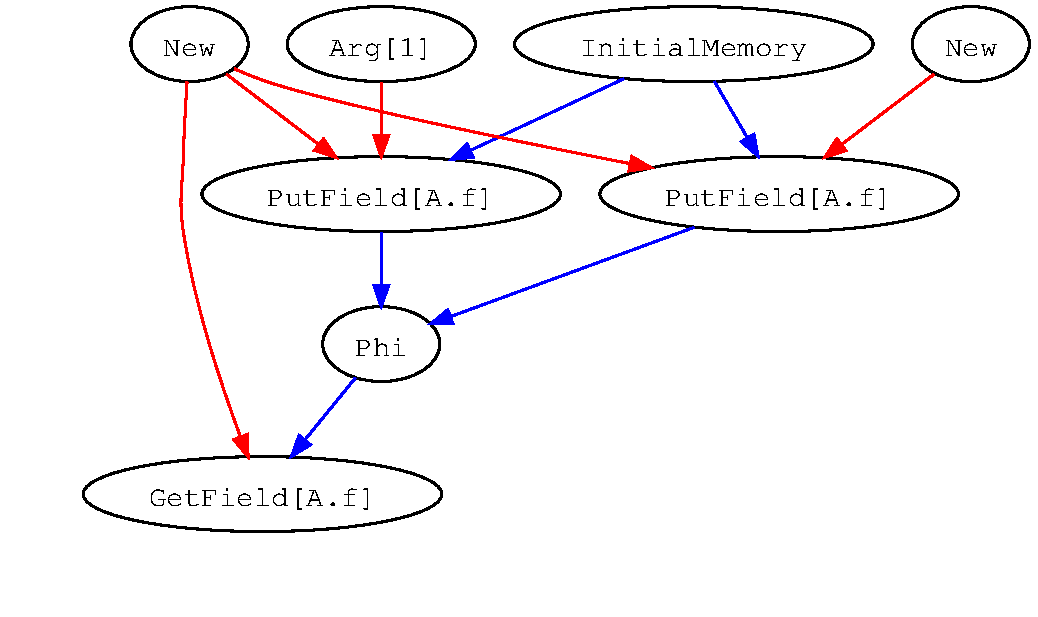
\includegraphics[width=\textwidth]{refmem_graph}
      \end{figure}
    \end{column}
    \begin{column}{0.33\textwidth}
      \begin{block}{Программа}
        \begin{algorithmic}[1]
          \State $a \gets \op{new}~\type{A}$
          \If{(\ldots)}
            \State $a.\field{f} \gets \op{new}~\type{A}$
          \Else
            \State $a.\field{f} \gets \op{arg}(1)$
          \EndIf
          \State $\op{return}~a.\field{f}$
        \end{algorithmic}
      \end{block}
    \end{column}
  \end{columns}

  \medskip
  \begin{center}
    \small
    Красные стрелки~--- зависимость по значению. \\
    Синие стрелки~--- зависимость по памяти.
  \end{center}

\end{frame}

\begin{frame}{Абстрактные объекты}

  \begin{center}
    \begin{minipage}[t]{0.70\textwidth}
      \begin{block}{Разные источники объектов}
        \begin{algorithmic}[1]
          \State $x \gets \op{new}(\type{T})$
            \Comment{$\pts{x} = \{O_1\}$}
          \State $y \gets \op{new}(\type{T})$
            \Comment{$\pts{y} = \{O_2\}$}
          \State $u \gets \op{getstatic}(\M_0, \sfield{T}{f})$
            \Comment{$\pts{u} = \{O_{global}\}$}
          \State $v \gets \op{arg}(1)$
            \Comment{$\pts{v} = \{O_{global}\}$}
        \end{algorithmic}
      \end{block}

    \end{minipage}
  \end{center}

  \medskip
  \centerline{$AbstractObjects = \{O_1, O_2, O_{global}\}$}

\end{frame}

\begin{frame}{Потоковые свойства}

  $\pts{expr} \subset AbstractObjects$

  \uncover<2->{\begin{align*}
    & \M = (\\
    & \quad \Mfield{fields} \subset
         AbstractObjects \times InstanceFields
           \times \powerset{AbstractObjects}, \\
    & \quad \Mfield{statics} \subset
         StaticFields \times \powerset{AbstractObjects}, \\
    & \quad \Mfield{shared} \subset AbstractObjects, \\
    & \quad \Mfield{escaped} \subset AbstractObjects\\
    & )
  \end{align*}}

\end{frame}

\begin{frame}{Пример потоковых функций}

  \[ x \gets \op{getstatic}(\M, \sfield{T}{f}) \Rightarrow \]
  \[
    \pts{x} = \M.\Mfield{shared} \cup \M.\Mfield{statics}(\sfield{T}{f}).
  \]

  \[ x \gets \op{getfield}(\M, a, \field{f}) \Rightarrow \]
  \[
    \pts{x} = \left( \bigcup_{O \in \pts{a}} \M.\Mfield{fields}(O,
    \field{f}) \right) \cup
    \begin{cases}
      \M.\Mfield{shared}, & \text{если } \pts{a} \cap
        \M.\Mfield{shared} \ne \emptyset; \\
      \emptyset, & \text{иначе}.
    \end{cases}
  \]

\end{frame}

\begin{frame}{Результаты анализа}

  Выражения ссылочного типа могут являться синонимами тогда и только
  тогда, когда их множества целей, вычисленные потоковым анализом, имеют
  непустое пересечение.

\end{frame}

\begin{frame}{Модель памяти языка Java}
  \begin{columns}[t]
    \begin{column}{.5\textwidth}
      \begin{block}{Чтение из \eng{volatile} поля}
        \begin{algorithmic}
          \State $a.\field{x} \gets 42$
          \State $\ldots$
          \State $t \gets b.\field{volatileField}$
          \State $\ldots$
          \State $x \gets a.\field{x}$
        \end{algorithmic}
      \end{block}
    \end{column}
    \begin{column}{.5\textwidth}
      \begin{block}{Чтение из обычного поля}
        \begin{algorithmic}
          \State $a.\field{x} \gets 42$
          \State $\ldots$
          \State $t \gets b.\field{normalField}$
          \State $\ldots$
          \State $x \gets \sout<2->{a.\field{x}}
                          \only<2->{\ 42}$
        \end{algorithmic}
      \end{block}
    \end{column}
  \end{columns}
\end{frame}

\begin{frame}{Практические результаты}

  \begin{itemize}
    \item<1-> Алгоритм анализа реализован в статическом компиляторе \java
              байткода в рамках проекта \eng{Excelsior Research Virtual
              Machine}.
    \item<1-> Реализованы следующие оптимизации:
          \begin{itemize}
            \item<2-> удаление избыточных чтений полей
            \item<3-> взрыв объектов и аллокация объектов на стеке
          \end{itemize}
  \end{itemize}

  \begin{columns}[t]
    \begin{column}{0.5\textwidth}
      \visible<2->{\begin{block}{Избыточные чтения}
        \begin{algorithmic}[1]
          \State $x.\field{f} \gets 42$
          \State $y.\field{f} \gets 37$
          \State $u \gets \sout<2->{x.\field{f}}
                          \only<2->{\ 42}$
        \end{algorithmic}
      \end{block}}
    \end{column}
    \begin{column}{0.5\textwidth}
      \visible<3->{\begin{block}{Взрыв объектов}
        \begin{algorithmic}[1]
          \State $\sout<3->{r \gets \op{new}~\type{Rect}(a, b)}$
          \State $u \gets \sout<3->{r.\op{area}()}
                        \ \only<3->{a \cdot b}$
        \end{algorithmic}
      \end{block}}
    \end{column}
  \end{columns}

\end{frame}

\begin{frame}{Результаты}

  Сделано следующее:
  \begin{itemize}
    \item изучены существующие алгоритмы анализа указателей и синонимов
    \item разработана схема выражения неявных зависимостей по памяти с помощью
          \M"=переменной
    \item разработан алгоритм, проводящий нечувствительный к потоку анализ над
          множеством операций, работающих с \M"=переменной
    \item реализован алгоритм в рамках проекта \eng{Excelsior
          Research Virtual Machine}
  \end{itemize}

  Получен диплом 1 степени на 51-ой международной научной студенческой
  конференции <<Студент и научно-технический прогресс>>.

\end{frame}

\begin{frame}{Дальнейшая работа}

  Планируется сделать следующее:
  \begin{itemize}
    \item внедрить в промышленный компилятор \eng{Excelsior JET}
    \item адаптировать для межпроцедурного анализа
  \end{itemize}

\end{frame}

\begin{frame}{Конец}
  \centerline{\huge Спасибо за внимание!}
\end{frame}

\begin{backup}

\begin{frame}{Запасные слайды}
  \centerline{\ldots}
\end{frame}

\begin{frame}{Представление потоковых свойств}

  \begin{block}{Внутреннее представление}
    \begin{algorithmic}
      \State $\M_0 \gets \op{initialmemory}$
        \visible<3->{\Comment{$\M_0 = \{\Mfield{fields}\colon}
          \{ O_1.\field{f} \colon \emptyset \}\}$}
      \State $a \gets \op{new}(\type{A})$
        \visible<2->{\Comment{$\pts{a} = \{O_1\}$}}
      \State
        \State $x_1 \gets \op{new}(\type{A})$
          \visible<2->{\Comment{$\pts{x_1} = \{O_2\}$}}
        \State $\M_1 \gets \op{putfield}(\M_0, a, \field{f}, x_1)$
          \visible<3->{\Comment{$\M_1 = \{\Mfield{fields}\colon}
            \{ O_1.\field{f} \colon \{ O_2 \} \}\}$}
      \State
        \State $x_2 \gets \op{arg}(1)$
          \visible<2->{\Comment{$\pts{x_2} = \{O_{global}\}$}}
        \State $\M_2 \gets \op{putfield}(\M_0, a, \field{f}, x_2)$
          \visible<3->{\Comment{$\M_2 = \{\Mfield{fields}\colon}
            \{ O_1.\field{f} \colon \{ O_{global} \} \}\}$}
      \State
      \State $\M_3 \gets \op{phi}(\M_1, \M_2)$
        \visible<3->{\Comment{$\M_3 = \{\Mfield{fields}\colon}
          \{ O_1.\field{f} \colon \{ O_2, O_{global} \} \}\}$}
      \State $y \gets \op{getfield}(\M_3, a, \field{f})$
        \visible<4->{\Comment{$\pts{y} = \{ O_2, O_{global} \}$}}
    \end{algorithmic}
  \end{block}

\end{frame}

\begin{frame}{Проблема многопоточности}

  \begin{columns}[t]
    \begin{column}{.5\textwidth}
      \begin{block}{Однопоточная программа}
        \begin{algorithmic}[1]
          \State $b \gets \op{new}~\type{A}$
          \State $b.\field{f} \gets 37$
          \State $\ldots$
          \State $\op{escape}(b)$
          \State $\ldots$
          \State $x \gets \sout<2->{b.\field{f}}
                          \only<2->{\ 37}$
          \State $\ldots$
          \State $y \gets \sout<2->{b.\field{f}}
                          \only<2->{\ 37}$
        \end{algorithmic}
      \end{block}
    \end{column}
    \begin{column}{.5\textwidth}
      \begin{block}{Многопоточная программа}
        \begin{algorithmic}[1]
          \State $b \gets \op{new}~\type{A}$
          \State $b.\field{f} \gets 37$
          \State $\ldots$
          \State $\op{escape}(b)$
          \State $\only<-3>{\ldots}
                  \only<4->{\op{while}~(\ldots)\ \ldots}$
          \State $x \gets \sout<3->{b.\field{f}}
                          \only<3->{\sout<4->{\ 37}}
                          \only<4->{\ b.\field{f}}$
          \State $\only<-4>{\ldots}
                  \only<5->{\op{while}~(\ldots)\ \ldots}$
          \State $y \gets \sout<3->{b.\field{f}}
                          \only<3->{\sout<4->{\ 37}}
                          \only<4->{\sout<5->{\ x}}
                          \only<5->{\ b.\field{f}}$
        \end{algorithmic}
      \end{block}
    \end{column}
  \end{columns}

\end{frame}

\begin{frame}{Проблема многопоточности}

  \begin{center}
    \begin{minipage}[t]{0.60\textwidth}
      \begin{block}{Многопоточная программа + \eng{JMM}}
        \begin{algorithmic}[1]
          \State $b \gets \op{new}~\type{A}$
          \State $b.\field{f} \gets 37$
          \State $\ldots$
          \State $\op{escape}(b)$
          \State $\only<-2>{\ldots}
                  \only<3>{\op{while}~(\ldots)\ \ldots}
                  \only<4->{\op{while}~(!\sfield{Data}{ready})\ \ldots}$
          \State $x \gets \sout<2->{b.\field{f}}
                          \only<2->{\sout<4->{\ 37}}
                          \only<4->{\ b.\field{f}}$
          \State $\only<-2>{\ldots}
                  \only<3->{\op{while}~(\ldots)\ \ldots}$
          \State $y \gets \sout<2->{b.\field{f}}
                          \only<2->{\sout<4->{\ 37}}
                          \only<4->{\ x}$
        \end{algorithmic}
      \end{block}
      \onslide+<4->{
        $\sfield{Data}{ready}$~--- статическое \eng{volatile} поле.}
    \end{minipage}
  \end{center}

\end{frame}

\begin{frame}{Некорректно синхронизованные программы}

  $\sfield{Shared}{data}$, $\sfield{Shared}{ready}$~--- обычные статические
  поля.

  \begin{columns}[t]
    \begin{column}{.5\textwidth}
      \begin{block}{Поток 1 <<Производитель>>}
        \begin{algorithmic}[1]
          \State $\sfield{Shared}{data} \gets \op{calc}(\ldots)$
          \State $\sfield{Shared}{ready} \gets \op{true}$
        \end{algorithmic}
      \end{block}
    \end{column}
    \begin{column}{.5\textwidth}
      \begin{block}{Поток 2 <<Потребитель>>}
        \begin{algorithmic}[1]
          \State $\alt<1>{\vphantom{A}\ldots}{result \gets \sfield{Shared}{data}}$
          \While{$(!\sfield{Shared}{ready})$}
            \State \ldots
          \EndWhile
          \State $\sout<2->{result \gets \sfield{Shared}{data}}$
        \end{algorithmic}
      \end{block}
    \end{column}
  \end{columns}

\end{frame}

\begin{frame}{Внутреннее представление сложных операций}

  \begin{columns}[t]
    \begin{column}{.5\textwidth}
      \begin{align*}
        a \gets \sfield{T}{f} & \\
        (\text{статическое \eng{volatile} поле}) & \\
        & \\
        \op{monitorenter}(\ldots) & \\
        & \\
        c \gets \op{invoke}(\method{foo}, p_1, \ldots, p_N) & \\
        & \\
        & \\
      \end{align*}
    \end{column}
    \begin{column}{.5\textwidth}
      \begin{align*}
        & \M_1 \gets \op{reload}(\M_0) \\
        & a \gets \op{getstatic}(\M_1, \sfield{T}{f}) \\
        & \\
        & \M_2 \gets \op{reload}(\M_1) \\
        & \\
        & \M_3 \gets \op{escape}(\M_2, p_1, \ldots, p_N) \\
        & \M_4 \gets \op{reload}(\M_3) \\
        & c \gets \op{shared}(\M_4) \\
      \end{align*}
    \end{column}
  \end{columns}

\end{frame}

\end{backup}

\end{document}

